\newpage
\section{Aufbau und Durchführung}
\subsection{Aufbau}
Eine schematische Darstellung des Versuchaufbaus ist in Abbildung \ref{fig:Aufbau} zu sehen.
Der hier verwendete Erbium:Faser-Laser TOPTICA hat eine Zentralwellenlänge von $1,55\,\si{\micro\meter}$ und eine Repetitionsrate von $75\,\si{\mega\hertz}$.
Das Laserlicht wird durch einen Strahlteiler in zwei gleich große Anteile aufgespalten, von denen einer über eine variable Verzögerungsstrecke läuft.
Beide Strahlen werden in einem Bismut-Borat-Kristall überlagert, in dem Summenfrequenzerzeugung bei zeitlicher und räumlicher Überlagerung entsteht.
Dabei werden die Strahlen so überlagert, dass sie hinter dem Kristall wieder räumlich auseinander laufen.
Der Anteil der Summenfrequenzerzeugung, der aus beiden einfallenden Laserstrahlen entsteht, erzeugt wegen der Impulserhaltung einen dritten Laserstrahl, der mittig verläuft und 
somit durch eine Irisblende seperat und untergrundfrei vermessen werden kann.
 
\begin{figure}[H]
    \centering\captionsetup{format=plain}
    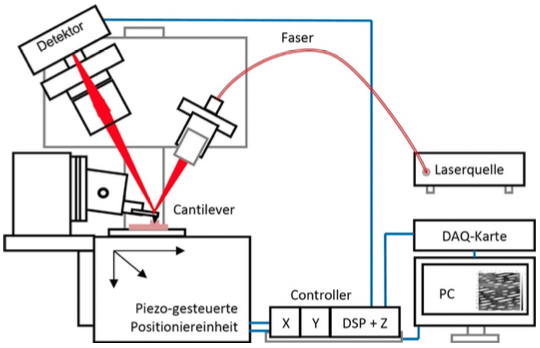
\includegraphics[width=0.9\textwidth]{bilder/Aufbau.png}
    \caption{Schematische Darstellung des Versuchsaufbaus. Entnommen aus \cite{anleitung}}
    \label{fig:Aufbau}
\end{figure}

Die Detektion der Intensität erfolgt mit einer Photodiode.
Um Hintergundrauschen zu minimieren wird die Lock-In-Technik verwendet.
Dabei wird das Laserlicht durch einen Chopper mit einer festgelegten Frequenz moduliert
und bei der Detektion durch einen Lock-In-Verstärker geleitet, der das Signal mit dem Referenzsignal des Choppers multipliziert und integriert.
Alternativ kann mittels eines Spektrometers vor dem Kristall das Spektrum des Laserlichts aufgenommen werden.

\subsection{Durchführung}
\label{sec:Durchfuehrung}

Zunächst wird die Pulsdauer des Lasers an sich bestimmt. Dazu wird 
zunächst der grobe Messbereich ermittelt und anschließend die Delay-Line in $1\,\si{\micro\meter}$-Schritten verändert.
Mit dem Spektrometer soll anschließend das Spektrum des Laserimpulses aufgenommen werden.

Als nächstes wird der Puls vermessen, wenn sich unterschiedliche Bandpassfilter im Strahlengang befinden,
die je eine Halbwertsbreite von $30\,\si{\nano\meter}$ und $12\,\si{\nano\meter}$ des resultierenden Spektrums um die Zentralwellenlänge von $1,55\,\si{\micro\meter}$
erzeugen.

Zuletzt soll der Einfluss von verschiedenen dispersiven Medien im Strahlengang untersucht werden.
Dazu steht ein Siliziumblock und SF11-Glasblöcke verschiedener Länge zur Verfügung.
Auch hier soll jeweils sowohl die Autokorrelation als auch das Spektrum bestimmt werden.